\input{../Common/commands}

\begin{document}

\graphicspath{ {../Common/images/} }
\input{../Common/map}
\graphicspath{ {images/} }


%----------------------------------------------------------------
% PAGE TITLE
% ----------------------------------------------------------------
\pgclrred
\title{\headerpres{Data Analysis: \\ Measuring Model Performance}}
\author{\vspace{3cm} Institute of Technology Tallaght}
\date{Department of Computing}
\maketitle
\newpage

% ----------------------------------------------------------------
% PAGE TABLE
% ----------------------------------------------------------------
\headerch{Basic Measures of Model Performance}
\begin{itemize}
\item How the performance of a model is measured depends on the context - each should be examined carefully and measures taken with specific goals in mind, not 'blindly'. Examples of context-defining activities:w
  \begin{itemize}
  \item building a general model for use with different data sets
  \item working out the profit resulting from the application of a model to a particular data set
  \end{itemize}
\item A useful concept to introduce here is the \textbf{confusion matrix}. This is the matrix of numbers - one for each target class (variable value) pair - representing the counts of instances of one class predicted as the other class. The top-left to bottom right diagonal of cells in the matrix contains correct prediction counts. The matrix size is $n \times n$ where $n$ is the number of classes.
  \newpage
  \item The confusion matrix below is the most commonly used, that for \textbf{binary prediction} (i.e. two target classes). The four counts are usually denoted \textbf{TP}, \textbf{FP}, \textbf{FN} and \textbf{TN}. The columns (p and n) contain the instances actually belonging to the positive and negative classes, respectively. The rows (Y and N) contain the instances predicted to be positive and those predicted to be negative, respectively.
    \begin{center}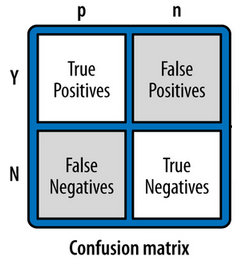
\includegraphics[width=0.2\textwidth]{7-2_confusion_matrix.png}\end{center}
  \item Various measures of performance can be derived from the confusion matrix:
    \begin{itemize}
    \item The measure most commonly used for quick assessment is \textbf{accuracy}, which measures the proportion of predictions that are correct, out of all the predictions made:
      $$ accuracy = \dfrac{TP+TN}{TP+FP+FN+TN}$$
      \newpage
    \item Also used are the '\textbf{rates}':
      \begin{itemize}
      \item true positive rate: $\dfrac{TP}{TP+FN}$, also called \textbf{specificity}
      \item false negative rate: $\dfrac{FN}{TP+FN}$
      \item true negative rate: $\dfrac{TN}{FP+TN}$, also called \textbf{sensitivity}
      \item false positive rate: $\dfrac{FP}{FP+TN}$
      \end{itemize}
      \twoex
    \item \textbf{Precision}, equal to $\dfrac{TP}{TP+FP}$, and \textbf{recall}, which is the same as the \emph{true positive rate} are used in calculating the F-measure:
      $$F-measure = 2\times \dfrac{precision \times recall}{precision + recall}$$
    \item \textbf{Positive predictive value} is the same as \emph{precision}
    \end{itemize}
    \newpage
  \item The value of accuracy is dependent on the particular mix of classes in the test dataset.
    
    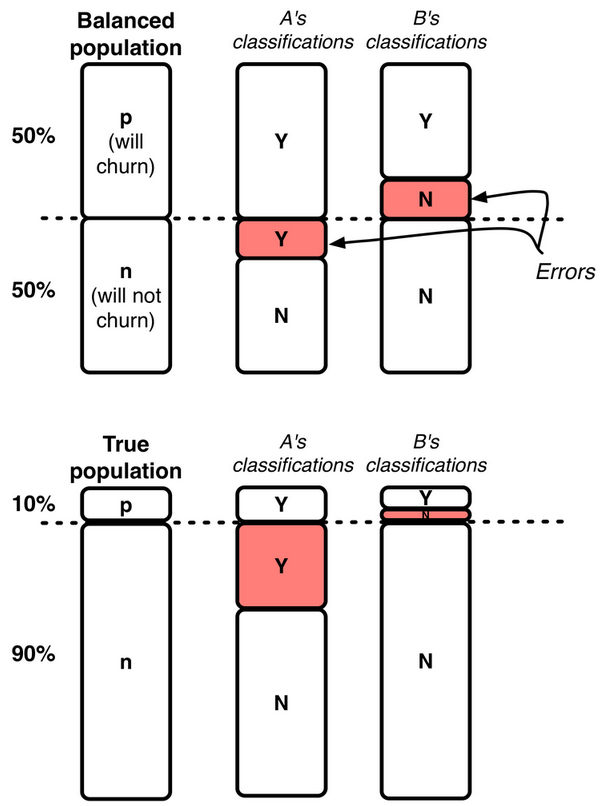
\includegraphics[width=0.25\textwidth]{7-1_nocap.png}
    \hspace{0.02\textwidth}
    \parbox[b]{0.65\textwidth}{In the picture model A predicts positives perfectly but predicts negatives with $60\%$ accuracy. B predicts negatives perfectly but predicts positives with $60\%$ accuracy. The result is that when the class mix is 50-50 the overall accuracy is the same for the two models but when the mix is 10-90 model B comes out as a lot better.}

    \item Accuracy does not take into account the 'cost' or 'benefit' of different outcomes, which can be considerably different. Take the example of the diagnosis of a serious illness. A false positive (diagnosis when no illness is present) would be an inconvenience but a false negative (an 'all-clear' when illness is presnet) could cost the patient her life.
\end{itemize}

\newpage

\headerch{Expected Value}
\begin{itemize}
\item Expected value in general is a value given to a situation that has a countable number of known outcomes with known probabilities. If the value of each outcome is also known or can be estimated, then the expected value is:

  $$EV=p(o_1)v(o_1)+p(o_2)v(o_2)+...+p(o_n)v(o_n)$$

  where $o_1$, $o_2$, ... $o_n$ are the outcomes, $n$ is the number of outcomes, $p(o_i)$ is the probability of outcome $o_i$ and $v(o_i)$ is the value of outcome $o_i$.
  \item In a data analytical context the values of $p(o_i)$ and $v(o_i)$ are determined as follows:
  \begin{itemize}
  \item the \textbf{probabilities} are estimated from the data, by building a model
  \item the \textbf{value} of each outcome must be determined using:
    \begin{itemize}
    \item general knowledge of the problem domain
    \item particular knowledge of the specific problem at hand
    \end{itemize}
  \end{itemize}

  \newpage

\item \emph{Expected value} can be calculated using the confusion matrix

  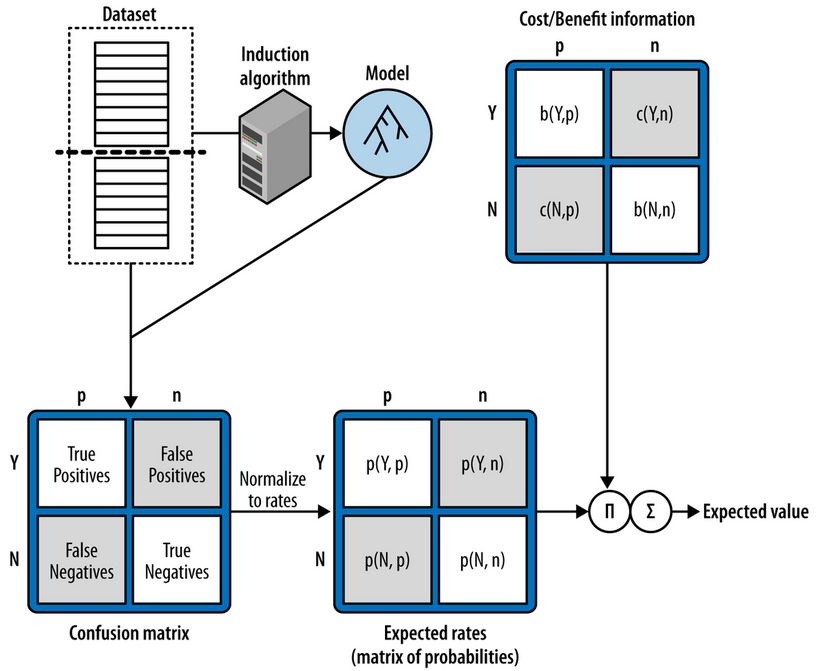
\includegraphics[width=0.4\textwidth]{7-2_nocap.png}\hspace{0.02\textwidth}
  \parbox[b]{0.5\textwidth}{The confusion matrix is \emph{normalised} i.e. the counts are converted to probabilities for the different outcomes. A matrix of the same dimensions is 'filled in' with cost and benefit values. The cell-for-cell multiplication of the matrices and summation of the values in the cells of the resulting matrix yields the \emph{expected value}. Beware of: \textbf{duplication of values} and \textbf{cost/benefit sign mix-ups}.}
  \begin{flalign*}
    expected\_value = &p(\bt{Y},\bt{p})b(\bt{Y},\bt{p})+p(\bt{N},\bt{p})c(\bt{N},\bt{p})+p(\bt{N},\bt{n})b(\bt{N},\bt{n})+p(\bt{Y},\bt{n})c(\bt{Y},\bt{n})
  \end{flalign*}
\item Another form of the same equation has the a priori probabilities of \bt{p} and \bt{n} separated out, for easy calculation for data sets with different class mixes
  \begin{flalign*}
    expected\_value = &p(\bt{p})[p(\bt{Y}|\bt{p})b(\bt{Y},\bt{p})+p(\bt{N}|\bt{p})c(\bt{N},\bt{p})]\\
    +&p(\bt{n})[p(\bt{N}|\bt{n})b(\bt{N},\bt{n})+p(\bt{Y}|\bt{n})c(\bt{Y},\bt{n})]
  \end{flalign*}

\end{itemize}

\newpage
\headerss{\underline{Example}}

{\small
Expected value can be used to determine whether some action would be viable and in what cases. In \textbf{targeted marketing} the action is the sending of marketing material to a particular person or class of person. When working with a predictive model that outputs the probability of a person or class of person responding to marketing, making a targeting decision based on the intuitive threshold of $0.5$ would not be very useful, as all the probabilities would be a lot lower than that threshold. In such cases, it is a lot more useful to look at the expected value (i.e. benefit) of targeting rather than use a simple threshold.
\begin{flalign*}
  expected\_value\_of\_targeting = p_R(x)v_R + [1 - p_R(x)]v_{NR}
\end{flalign*}
In the formula above, $p_R(x)$ is the probability of $x$ (a person or a class of person) responding, $v_R$ is the benefit of a response and $v_{NR}$ is the value (which will be negative) of a non-response. Let's say that the targeted marketing is for a product that would bring a profit of \euro$100$ if the targeted person bought it (responding to the marketing action) and that the price of creating and sending the material is \euro$1$ per address. Then we would have:
\begin{flalign*}
  v_R = \text{\euro}100 - \text{\euro}1 = \text{\euro}99,\qquad v_{NR} = -\text{\euro}1
\end{flalign*}
For the values above, the expected value of targeting is greater than 0 when $p_R > 0.01$. Thus we may decide to target any person for whom this condition is met, expecting that such action would, on average, be of benefit.

}

\newpage

\headerch{Baseline models}

For the assessment of a model to make sense, we must compare it to some other reference model.
\begin{itemize}
\item Random model - easy to beat but good for initial exploration
\item Meteorological prediction models have two important baselines: persistence and climatology
\item Classification - majority class
\item Regression - average or median, also averages across different data subsets
\item Single feature prediction - simplest but often good as a first model (decision \emph{stump} as opposed to tree)
\item Single datasource - rather than many integrated data sources
\item Baseline based on some experiential wisdom e.g. increased account activity in fraud detection
\end{itemize}

\newpage

\headerch{Model performance visualisation}

\begin{itemize}
\item Ranking of items - this is something that can be achieved with most classification models, whether they produce probabilities (e.g. Na\"ive Bayes) or values between 0 and 1 that do not actually correspond to probabilities (logistic regression). The data instances are simply ranked from the 'most probable' to the 'least probable' based on the model output.
  
  \begin{center}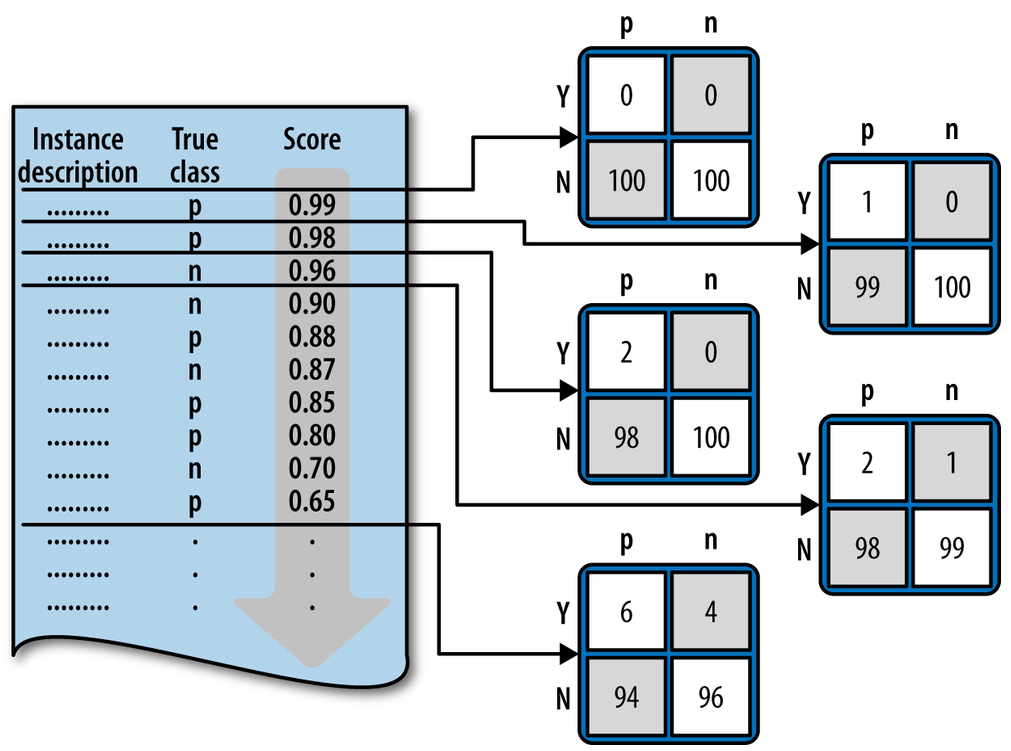
\includegraphics[width=0.3\textwidth]{8-1_nocap.png}\end{center}

\item Why rank instead of classify? Because the standard decision boundary of 0.5 would not make sense for many applications. E.g. the earlier described direct marketing example and the boundary that would make sense is \textbf{not known in advance}.
\item Ranking allows the decision boundary to be determined depending on profit and budget
\newpage

\item Profit curves 
 
  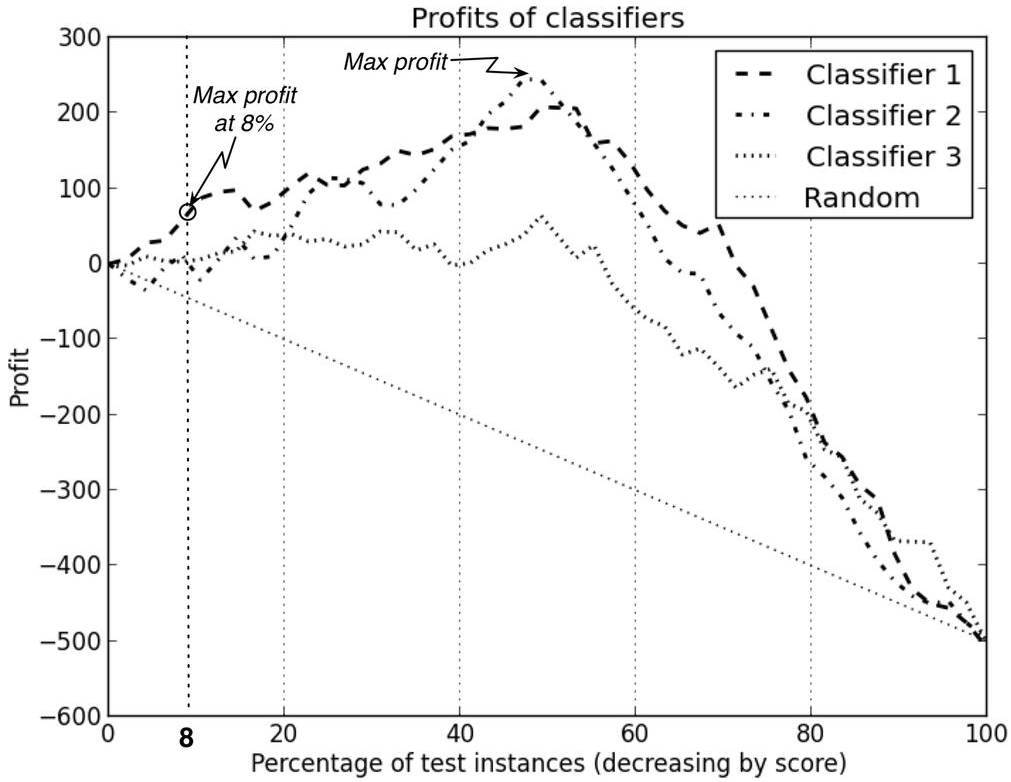
\includegraphics[width=0.4\textwidth]{8-2_nocap.png}\hspace{0.01\textwidth}
  \parbox[b]{0.54\textwidth}{\small Profit curves provide information about the performance of classifiers and can help with determining the best binary decision boundary for a data set and given classification methods. A profit curve can be used when the \textbf{prior probabilities of the classes} and the \textbf{cost-benefit matrix} are stable across all data sets (those used to build the prediction model and those to be classified). Examples of questions that a profit curve would help answer are ''Which one of three classifiers is the best one to use if the budget is limited (e.g. to target-marketing $8\%$ of unknown subjects)?'' [Classifier 1 in the picture] or it might be ''Which one of the three classifiers, when used to rank the new subjects, would bring about the hightest profits with an unlimited budget?'' [Classifier 2 in the picture]}
  
  \vspace{-0.5ex}
  {\small The x-axis of a profit curve represents the percentage of data instances that is found above the decision boundary as the boundary is moved, instance by instance, down the ranked (e.g. by probability to respond to targeted marketing) list of instances in a training set. The y-axis shows the profit that results from the boundary being placed at the different points in the list (e.g. targeted marketing is directed at subjects above the line). Initially the profit rises more steeply (as a working classifier would rank positives, bringing profit, at the top) and starts falling once many negatives start being included above the boundary (these are false positives, incurring cost). In the picture, classification model 1 is good at identifying the instances with the highest probabilities, while classification model 2 has better performance in identifying the most highly probable $50\%$ of instances. \par}

\newpage

\item Receiver Operating Characteristics (ROC) graphs \& curves and area under the curve (AUC)
  
  \fbox{\parbox[b]{0.93\textwidth}{\tiny \emph{ROC has its origins in WW2, whence it was used as a measure of radar performance.}}}
  
  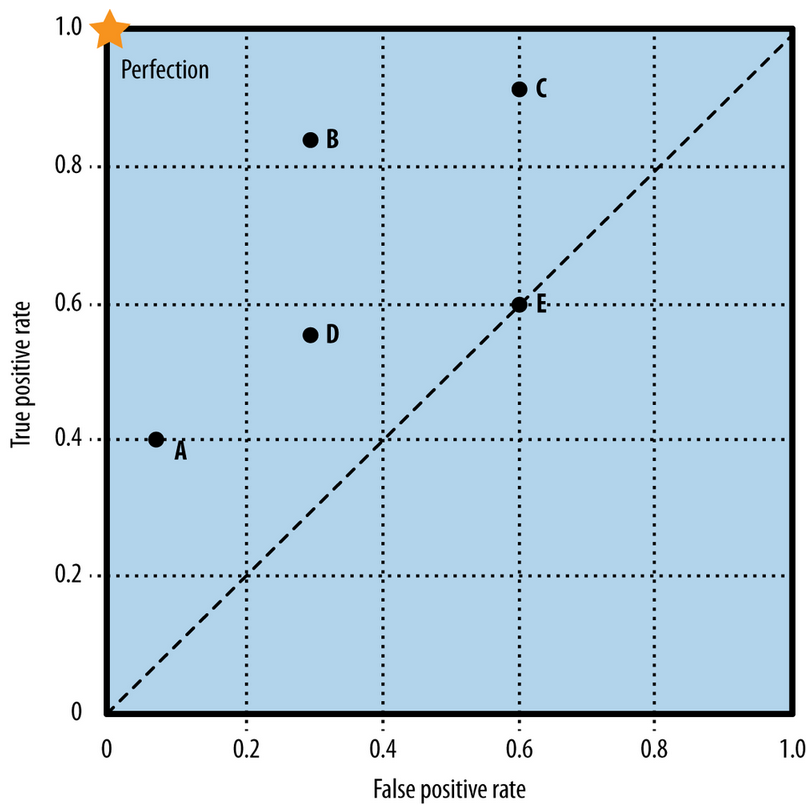
\includegraphics[width=0.35\textwidth]{8-3_nocap.png}\hspace{0.01\textwidth}\parbox[b]{0.23\textwidth}{\small Each point in an ROC graph [left] corresponds to a contiguous portion, extending from the top, of a ranked instance list. The x-component of the point is the part (out of 1) of the data set's \textbf{true positives} contained in the list portion corresponding to the point. The y-component is the same part for \textbf{false positives}.}\hspace{0.01\textwidth}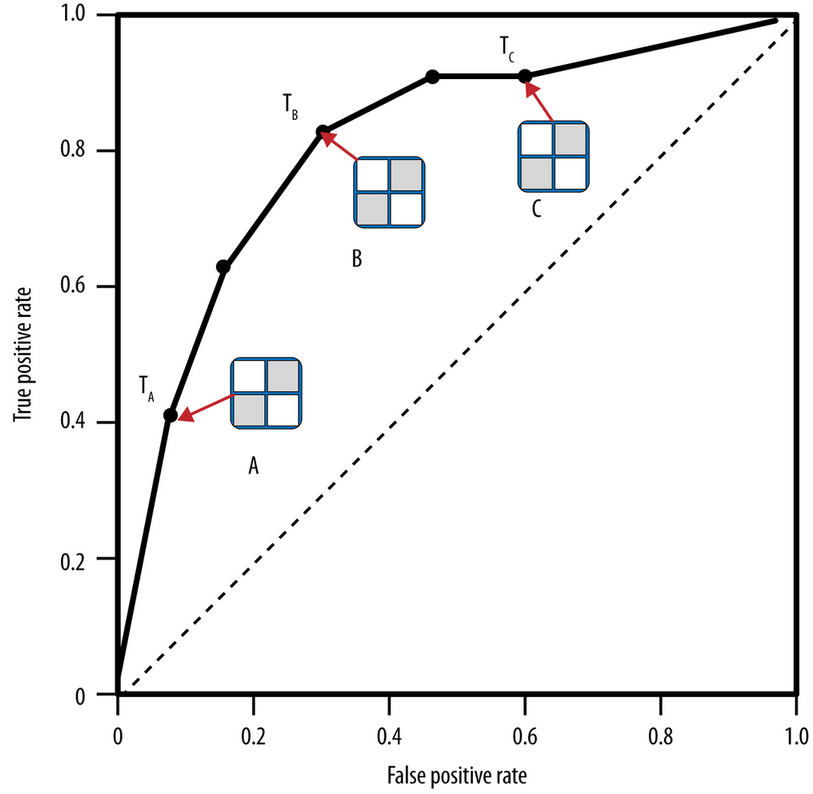
\includegraphics[width=0.35\textwidth]{8-4_nocap.png}
  
  \vspace{-0.5ex}
  {\small An ROC curve [right] is a systematic plot of points like those in the ROC graph together with a connecting line, for all possible contiguous portions, extending from the top, of the ranked instance list (starting with an empty list and concluding with the entire list).

  \vspace{-0.5ex}
    ROC curves provide a measure of classifier performance that is \textbf{independent of class priors and of the cost-benefit matrix}. The closer the curve is to the two-straight-segment-line (0,0)-(0,1)-(1,1) the better the performance of the classifier, indicating more positives placed towards the top of the ranked list. The area under the ROC curve (AUC) provides a numeric measure of this quality: a value of 1 indicates a perfect classifier while a value of 0.5 correpsonds to random classification.
    
    }
  \newpage

\item Cumulative response and lift curves
 
  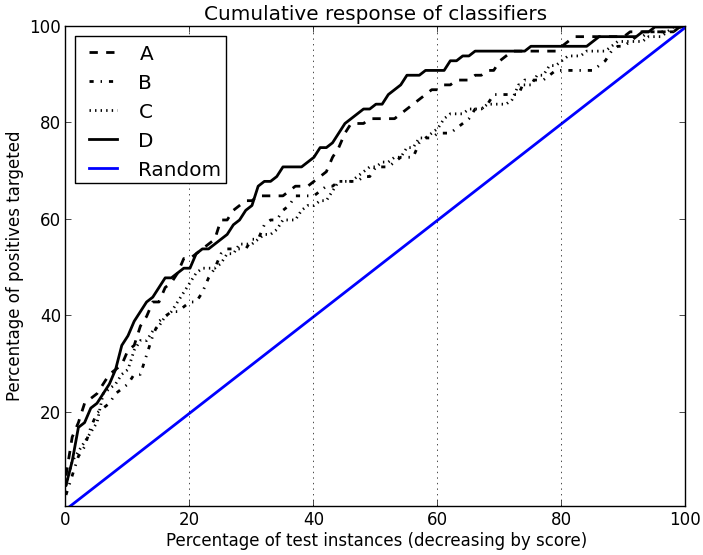
\includegraphics[width=0.4\textwidth]{8-6_nocap.png}\hspace{0.15\textwidth}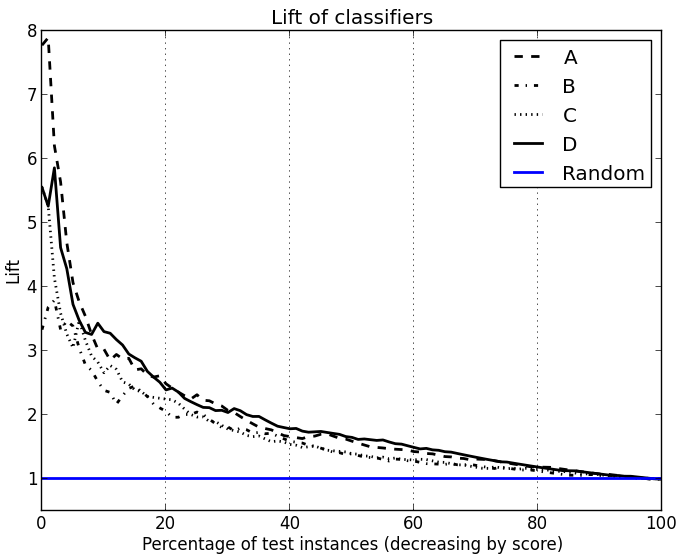
\includegraphics[width=0.4\textwidth]{8-7_nocap.png}

  {\small  A \textbf{cumulative response curve} [left] is similar to an ROC curve but the x-axis, instead of representing the part of all false positives found in the cut-off portion of the ranked instance list, represents the percentage of the entire list of instances that is contained in the portion of the list above the cut-off point. This means that the shape of the cumulative response curve, while somewhat easier to understand for a non-technical audience, depends on the class priors and is thus not as pure a measure of a classifier's performance. 

   Every cumulative response curve (CRC) has a corresponding \textbf{lift curve} [right] which has the same values on the x-axis as the CRC and shows the ratios of the CRC y-values to the CRC y-values for random classification (this means that the lift curve for random classification is a constant 1).
    
  }
  
\newpage
\end{itemize}

\headerss{\underline{Example}}

KDD Cup 2009 - French Telecom company Orange data

  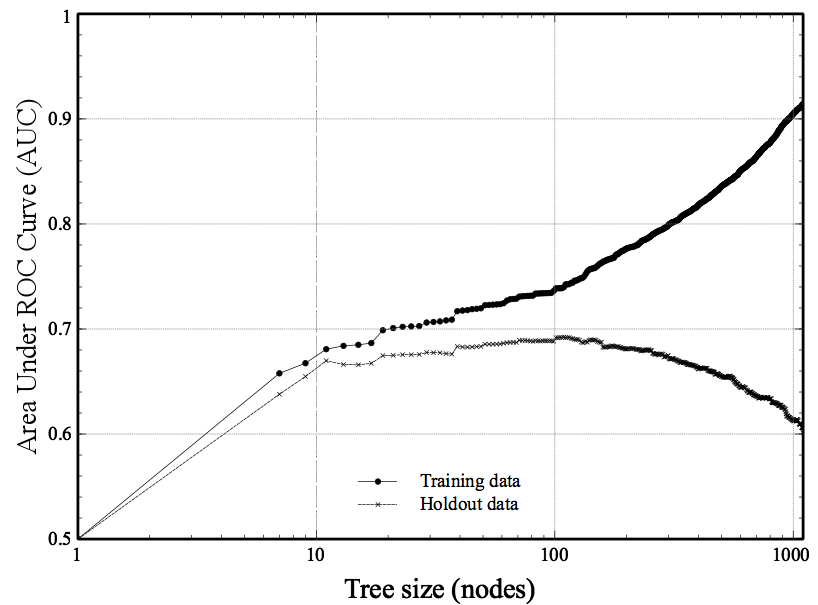
\includegraphics[width=0.3\textwidth]{8-8_nocap.png}\hspace{0.02\textwidth}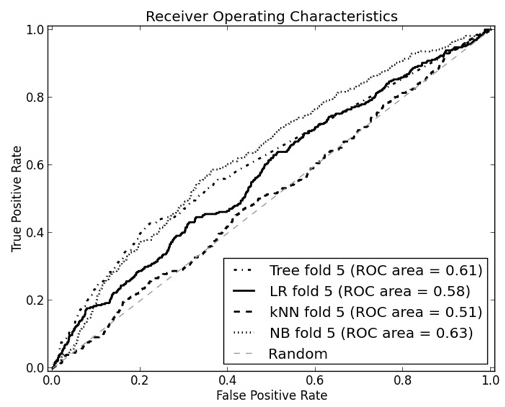
\includegraphics[width=0.3\textwidth]{8-9_nocap.png}\hspace{0.02\textwidth}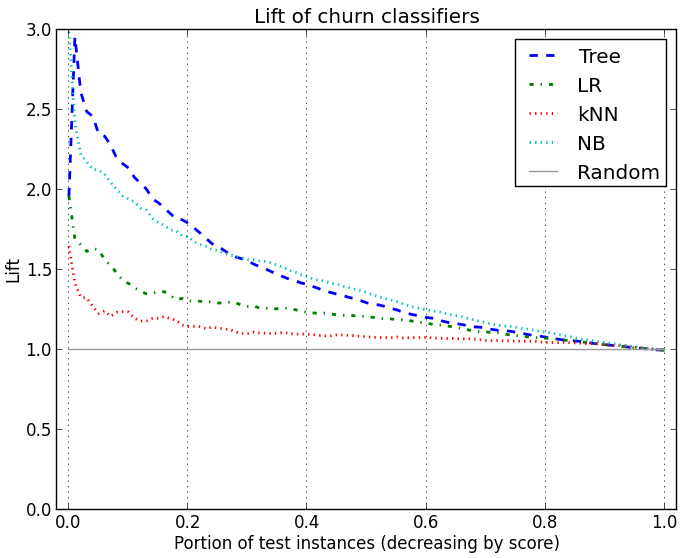
\includegraphics[width=0.3\textwidth]{8-10_nocap.png}

  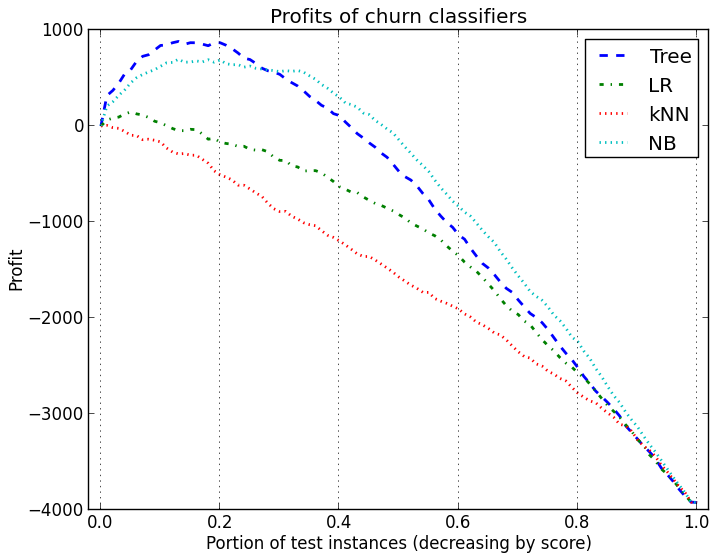
\includegraphics[width=0.3\textwidth]{8-11_nocap.png}\hspace{0.02\textwidth}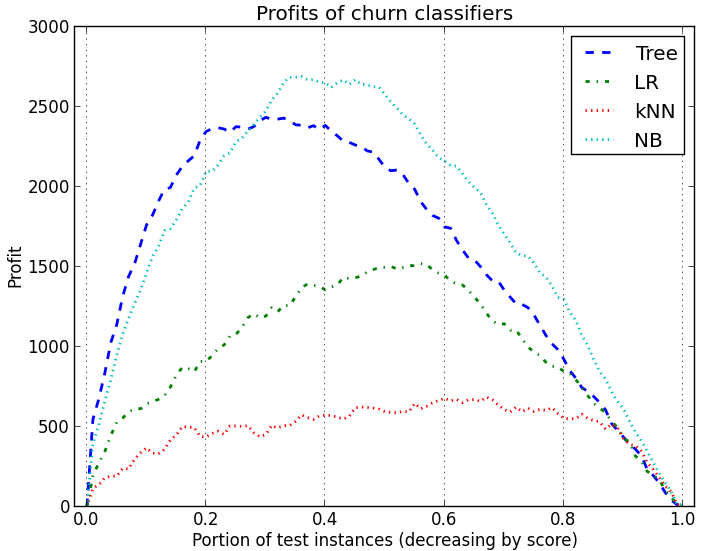
\includegraphics[width=0.3\textwidth]{8-12_nocap.png}\hspace{0.02\textwidth}
  \begin{minipage}[b]{0.36\textwidth}
    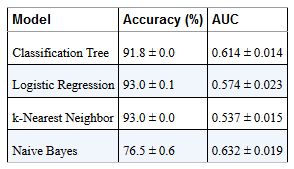
\includegraphics[width=0.55\textwidth]{orange_accuracy_table.png}\hspace{0.02\textwidth}\scalebox{0.5}{\parbox[b]{0.7\textwidth}{\small Although kNN produces considerably better accuracy than the Na\"ive Bayes classifier, the confusion matrices and diagrams show that kNN acts practically as a base-rate classifier and is in fact not the better of the two models.

      }}

    \vspace{-1.5ex}
    \scalebox{0.5}{\small Na\"ive Bayes Confusion Matrix\phantom{---------------}k-NN Confusion Matrix}

    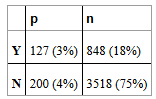
\includegraphics[width=0.4\textwidth]{nb_cm.png}\hspace{0.1\textwidth}
    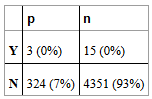
\includegraphics[width=0.4\textwidth]{knn_cm.png}
    
  \end{minipage}
  



\newpage
%----------------------------------------------------------------
% PAGE REFERENCES
% ----------------------------------------------------------------
\headersec{References}

\textbf{[DSB]} \emph{Data Science for Business: What you need to know about data mining and data-analytic thinking}, by Foster Provost and Tom Fawcett, O'Reilly Media, 2013. 





\end{document}

